\noindent Quarter-wavelength attenuators (both series and shunt arrangements) are microwave attenuators that use a $\lambda/4$ inverter. These types of attenuators only provide matching at the input port \cite{pin_diode_designer_handbook}.

  \begin{figure}[ht]
    \centering
    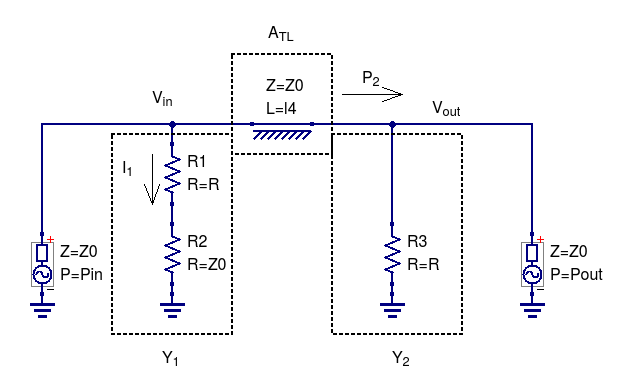
\includegraphics[width=10cm]{./images/qw-series-attenuator-schematic.png}
    \caption{Quarter wavelength series attenuator}
    \label{fig:qw-series-attenuator-schematic}
  \end{figure}

\noindent The design equations of the quarter-wavelength series attenuator can be derived using cascade analysis:

\begin{equation}
	Y_1 = \begin{pmatrix}
				1 & 0\\
				\frac{1}{R + Z_0} & 1
		  \end{pmatrix}
\end{equation}

\begin{equation}
	A_{TL} = \begin{pmatrix}
				cosh(\gamma \cdot l) & Z_0 \cdot sinh(\gamma \cdot l)\\
				\frac{1}{Z_0} \cdot sinh(\gamma \cdot l)  & cosh(\gamma \cdot l)
		     \end{pmatrix}
\end{equation}

\noindent where $\gamma = \alpha + j \cdot \beta$ is the propagation constant. Since the $\lambda/4$ transmission line is supposed to be lossless, then $\gamma = j \cdot \beta = j \cdot \frac{2 \cdot \pi}{\lambda}$ and, consequently:

\begin{equation}
	A_{TL} = \begin{pmatrix}
				0 & j \cdot Z_0\\
				\frac{j}{Z_0}  & 0
		     \end{pmatrix}
\end{equation}

\noindent The ABCD matrix of the $Y_2$ block is simply:

\begin{equation}
	Y_{2} = \begin{pmatrix}
				1 & 0\\
				\frac{1}{R}  & 1
		     \end{pmatrix}
\end{equation}

\noindent The overall ABCD matrix is given by:

\begin{equation}
	A_{QW_{series}} = Y_1 \cdot A_{TL} \cdot Y_2 = j \cdot Z_0 \cdot \begin{pmatrix}
				\frac{1}{R} & 1\\
				\left( \frac{1}{R \cdot (R + Z_0)} + \frac{1}{Z_0^2} \right)  & \frac{1}{R + Z_0}
		     \end{pmatrix}
\end{equation}

\noindent Using the conversion formulae between ABCD and S parameters \cite{pozar2012microwave}:

\begin{equation}
	S = \begin{pmatrix}
				0 & -j \cdot \frac{R}{R + Z_0}\\
				-j \cdot \frac{R}{R+Z_0}  & \frac{Z_0^2}{(R + Z_0)^2}
		\end{pmatrix}
\end{equation}

\noindent Thus, the attenuation (in dB) can be expressed in terms of R and $Z_0$ as follows:

\begin{equation}
	\alpha = -20 \cdot log_{10} \left( \frac{R}{R+Z_0}\right)
\end{equation}

\noindent Then,

\begin{equation}
	R = \frac{Z_0}{10^{\frac{\alpha}{20}} - 1}
\end{equation}

\noindent The impedance inversion property of the $\lambda$/4-transmission line holds in the vecinity of the center frequency. The general (broadband) expressions for the S-parameters of the quarter wavelength attenuators are much more complex and numeric S-parameter simulation analysis is more convenient for the analysis.

\noindent The impedance seen at the output port is given by:

\begin{equation}
	Z_{out} = \frac{R^2 \cdot Z_0 + 2 \cdot R \cdot Z_0^2}{R^2 + 2 \cdot R \cdot Z_0 + 2 \cdot Z_0^2}
\end{equation}

\noindent The power dissipated in the resistors at the center frequency ($f_c$) is calculated as follows:

\begin{equation}
	P_{R1} = P_{R3} = I_1^2 \cdot R_1 = \left( \frac{V_{in}}{R_1 + Z_0}\right)^2 \cdot R_1= P_{in} \cdot \left( \frac{ Z_0}{(R_1 + Z_0)^2} \right) \cdot R_1
\end{equation}

\begin{equation}
	P_{R2} = P_{in} \cdot \left( \frac{Z_0}{R_1 + Z_0} \right)^2
\end{equation}

   \begin{figure}[ht]
    \centering
    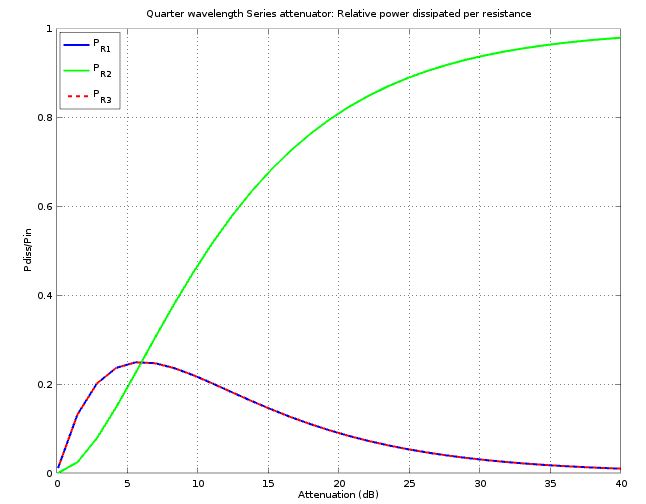
\includegraphics[width=10cm]{./images/qw-series-relative-power-dissipation-50-Ohm.png}
    \caption{Power dissipated in the resistors of the quarter wavelength series attenuator with respect to the input power. $Z_{in} = Z_{out} = 50 \Omega$}
    \label{fig:qw-series-att-relative-power-dissipation-50-Ohm}
  \end{figure}